\documentclass[12pt,a4paper,tablecaptionabove]{scrartcl} 
\usepackage{ngerman}   % neue deutsche Rechtschreibung (Trennregeln ...)
\usepackage[utf8]{inputenc} % UTF8 Zeichenkodierung, falls das nicht
                            % funktioniert
                            % \usepackage[latin1]{inputenc} verwenden
\usepackage[T1]{fontenc} % Deutsche Umlaute und so
\usepackage{ae}        % Schriften für Adobe Acrobat
\usepackage{textcomp}  % mehr Sonderzeichen
\usepackage{calc}      % Paket für die Berechnung von Längen
\usepackage{color}     % Farbiger Text etc.
\usepackage{graphicx}  % importieren von Graphiken
\usepackage{subfigure} % Mehrere Abbildungen in einer figur
\usepackage{booktabs}  % für schöne Tabellen
\usepackage[numbers]{natbib}    % Für Literaturverzeichnis nach DIN 1505
\usepackage{scrpage2}  % Kopf- und Fusszeilen
\usepackage{tabularx}  % Tabellen auf Textbreite einpassen
\usepackage{verbatim}  % Programmcode angeben
\usepackage{listings}  % Programmcode mit mehr Optionen
\usepackage{hyperref}  % Links innerhalb des PDF-Files
\usepackage{subscript} % Hoch-, Tiefstellen
\usepackage{float} % das die cheibe Grafike au döt bliibe, wo si sötte
\usepackage{pdflscape} % Hoch-, Querformat
\usepackage{a4wide} % Textbreite





% Titel definieren
\title{Messung und Modelierung der Evapotranspiration}
\author{Debora Jäckel\\Simon Roth\\Gabriela Schär \\Alexandra Schuler}
\date{\today{}}

\begin{document}


% Schriften für Abbildungsbeschriftungen
\renewcommand*{\capfont}{\normalfont}
\renewcommand*{\caplabelfont}{\sffamily\bfseries}


% Kopf- und Fusszeilen definieren
\pagestyle{scrheadings}

% Dynamische Kopfzeilen
%\automark[section]{chapter}

% Statische Kopfzeilen
\ihead{Labor II}
\chead{ }
\ohead{Experiment 4}
\ifoot{}
\cfoot{ }
\ofoot{\pagemark}

% Trennstriche zwischen Kopf- und Fusszeile
\setheadsepline{0.5pt}
\setfootsepline{0.5pt}

% Schrftart für Kopfzeile
\setkomafont{pagehead}{\normalfont\slshape}

% Titel ausgeben
\maketitle

\newpage

\begin{abstract}

Die Evapotranspiration ist ein wichtiger Parameter bei der Untersuchung des Wasserkreislaufes, der Modellierung von Einzugsgebieten, der Optimierungen in der Landwirtschaft und in vielen anderen Bereichen. Sie kann entweder direkt aus Lysimeterdaten berechnet oder anhand von empirischen Modellen und meteorologischen Daten modelliert werden. In diesem Versuch werden die empirischen Methoden von Penman-Monteith, Turc und Ivanov verwendet. Alle Daten werden mit MATLAB prozessiert und dargestellt.

In einem ersten Teil wird die Korrelation zwischen der realen Evapotranspiration und den meteorologischen Grössen untersucht. Dabei ist zu erkennen, dass besonders die Globalstrahlung einen entscheidenden Einfluss auf die Evapotranspirationsrate hat und die Windgeschwindigkeit in der Schweiz vernachlässigbar ist.

In einem zweiten Teil werden die verschiedenen Methoden zur Bestimmung der potentiellen Evapotranspiration miteinander verglichen. Die modellierten Evapotranspirationsraten liegen bei allen Modellen in derselben Grössenordnung, wobei in der täglichen Auflösung die Methode nach Turc und Ivanov eine grössere Abhängigkeit von den meteorologischen Parametern Globalstrahlung, Temperatur und relative Luftfeuchtigkeit zeigen als dies mit der Penman-Monteith Methode der Fall ist.

Mit einem Pflanzenfaktor kann die potentielle Evapotranspiration für jede spezifische Pflanzenart bestimmt werden. In diesem Versuch werden die potentiellen Evapotranspirationsraten von Raps und Weizen miteinander verglichen. Diese verhalten sich im jährlichen Verlauf sehr ähnlich, ausser dass die maximale reale Evapotranspiration des Weizens ein Monat nach jener von Raps erreicht wird.

In einem weiteren Teil wird für jede Methode eine Sensitivitätsanalyse durchgeführt. Dabei zeigen bei der Methode nach Penman-Monteith und Ivanov alle Parameter eine etwa gleich grosse Sensitivität. Bei der Turc-Methode ist die relative Luftfeuchtigkeit der sensitivste Faktor.

\end{abstract}

\newpage
% Inhaltsverzeichnis
\tableofcontents
% Neue Seite
\newpage


\section{Einleitung}

Wasser verlässt ein Gebiet in dem es entweder als Oberflächenabfluss, Basisabfluss oder Grundwasser abfliesst, oder es Verdunstet. Wird das Wasser von der Bodenoberfläche verdunstet, spricht man von Evaporation. Verdunstet es von Pflanzenoberflächen, so ist dies die Transpiration. Da es schwierig ist, diese beiden Messgrössen technisch voneinander zu trennen, werden sie zu einer Grösse, der Evapotranspiration, zusammengefasst.

In diesem Versuch geht es nun darum, Evapotranspiration mit verschiedenen Modellen zu bestimmen. Für die Hydrologie ist es wichtig, die Evapotranspiration zu kennen, da sie ein wichtiger Bestandteil in der Wasserbilanz eines Einzugsgebiets ausmacht.

Es gibt verschiedene Methoden, die Evapotranspiration zu bestimmen. Zum einen gibt es empirische Modelle, zum anderen kann die Evapotranspiration auch mit Lysimetern gemessen werden. Empirische Modelle werden entwickelt, in dem die Evapotranspiration als Funktion von meteorologischen Variablen beschrieben wird. Es handelt sich dabei um meteorologische Variablen, die einen starken Einfluss auf die Evaporation haben, zum Beispiel Lufttemperatur, globale Strahlung, Sonnenscheindauer, Luftfeuchtigkeit, etc. Dazu wird die Evapotranspiration in einem Versuchsgebiet gemessen und mit den Meteodaten in Verbindung gesetzt. Da diese Modelle für bestimmte Standorte mit zugehörigen Eigenschaften entwickelt werden, sind sie nicht immer auf andere Standorte übertragbar und können nicht als allgemein gültig angenommen werden.

Für die Auswertungen stehen Lysimeterdaten von der Forschungsanstalt Agroscope Reckenholz-Tänikon ART und Meteodaten der ANETZ Station in Reckenholz zur Verfügung. Mit den Lysimeter- und den Meteodaten kann die Evapotranspiration direkt berechnet werden. Für die Modellierung mit der FAO Penman-Monteith-, Turc- und Ivanov-Methode werden nur die Meteodaten verwendet.

Ziel des Versuchs ist es, zu verstehen, was die Evapotranspiration ist und welche Methoden es gibt, diese zu bestimmen.
\section{Methode}
Für die Bestimmung der Evapotranspiration werden die Lysimeter- und Meteodaten mit MATLAB prozessiert. Da die Meteodaten in UTC und die Lysimeterdaten in MEZ vorliegen, müssen die Datensätze zuerst an eine Zeit angepasst werden. Zudem müssen die Einheiten so angepasst werden, dass sie auf die jeweiligen Berechnungsformeln passen.
\subsection {Lysimeter}

Ein Lysimeter ist eine Anlage, die zur Analyse von Wasser- und Stofftransport durch den Boden dient. Es besteht aus einem zylindrischen Topf, der mit Erde gefüllt ist. Am unteren Ende befindet sich ein Auslass für das versickerte Wasser und am Rand befinden sich auf verschiedenen Höhen diverse Messsonden. Wenn das Lysimeter auf einer Waage steht, kann zusätzlich die Gewichtsveränderung und somit der Wasserinput durch Niederschlag und der Wasserverlust durch die Evapotranspiration gemessen werden. Die Abbildung \ref{fig:lysimeter_ART}  zeigt die oberirdische Ansicht der Lysimter der ART. Eine Beschreibung der Komponenten der Lysimeter ist in der Abbildung \ref{fig:lysimeter_schema} zu sehen.\\

\begin{figure}[H]
\centering
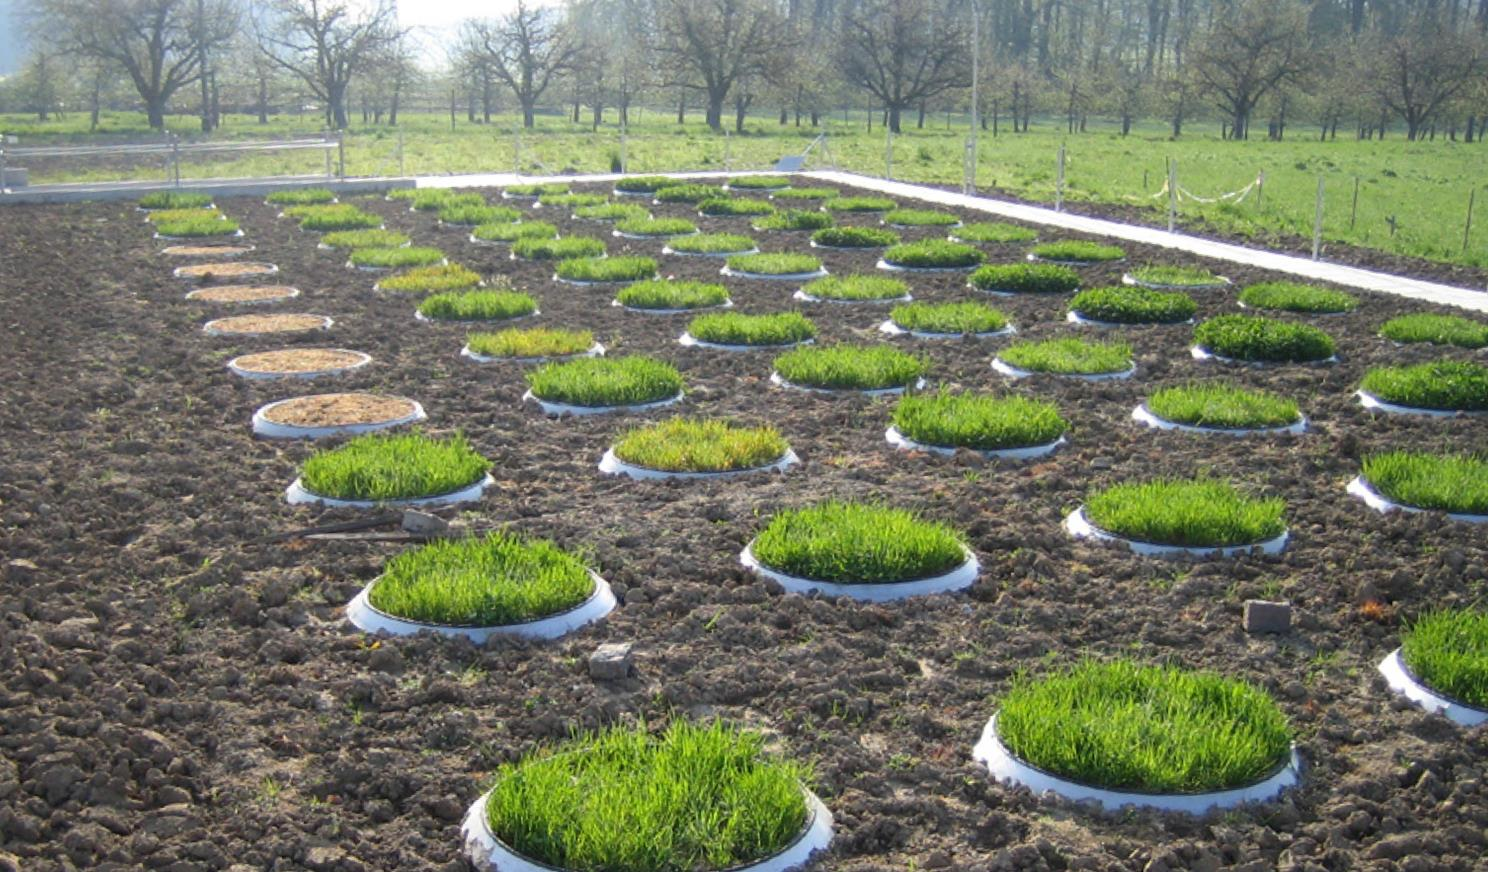
\includegraphics[width=0.8\textwidth]{figures/lysimeter_ART.jpg}
\caption{Lysimeteranlage der Forschungsanstalt Agroscope Reckenholz-Tänikon ART aus \cite{art}}
\label{fig:lysimeter_ART}
\end{figure}
 
\begin{figure}[H]
\centering
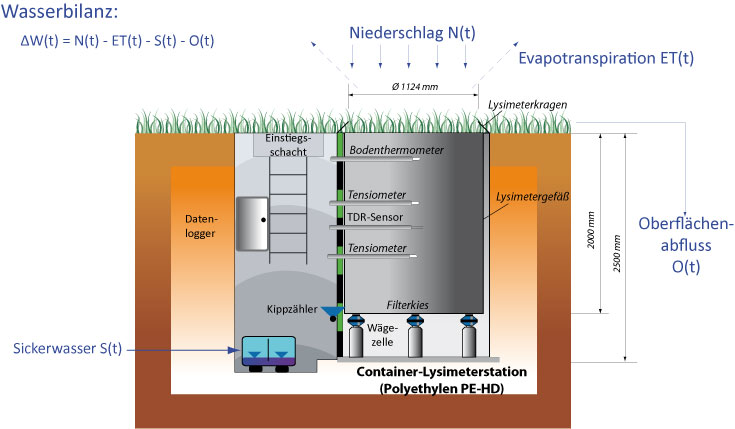
\includegraphics[width=0.8\textwidth]{figures/lysimeter_schema.jpg}
\caption{Schematische Darstellung eines Lysimeters aus \cite{ugt}}
\label{fig:lysimeter_schema}
\end{figure}


Zur Berechnung der Evapotranspiration mittels Lysimeterdaten wird die Bilanzformel (\ref{eq:wasserbilanz}) verwendet.


\begin{equation}
\label{eq:wasserbilanz}
AET=P-SW-\Delta W
\end{equation}
\begin{table}[H]
\centering
\begin{tabular}{ll}
AET& Reale Evapotranspiration [H/T$^{-1}$]\\
P& Niederschlagsrate  [H/T$^{-1}$]\\
SW & Sickerwasserrate  [H/T$^{-1}$]\\
$\Delta W$ & Änderung der Wasserspeichers  [H/T$^{-1}$]\\
\end{tabular}
\end{table}


Die Änderung des Wasserspeichers wird aus der Gewichtsdifferenz des Lysimeters berechnet (\ref{eq:gewichtsänderung}).


\begin{equation}
\label{eq:gewichtsänderung}
\Delta W=\frac{\Delta m}{\rho_{Wasser}* A}
\end{equation}
\begin{table}[H]
\centering
\begin{tabular}{ll}
$\Delta W$ & Änderung der Wasserspeichers  [H/T$^{-1}$]\\
$\Delta m$ & Gewichtsänderung [kg]\\
$\rho_{Wasser}$ & Dichte des Wassers [kg/m$^3$]\\
A & Oberflläche des Lysimeters [m$^2$]
\end{tabular}
\end{table}

 Zur Bestimmung der Niederschlagsrate werden die Daten eines Niedeschlagsmessgeräts verwendet. Die Sickerwasserrate wird aus de


\subsection{FAO Penman-Monteith-Methode}

Die Penman-Monteith-Methode kombiniert die beiden Ansätze der Massenbilanz und der Energiebilanz. Alle in der Formel enthaltenen Parameter können entweder direkt gemessen oder dann aus meteorologischen Daten berechnet werden. Die Methode impliziert, dass der aerodynamische und der Oberflächenwiderstand von der Oberflächenbepflanzung abhängig sind [vgl.\,Abb.\,\ref{fig:widerstand}]. 

\begin{figure}[H]
\centering
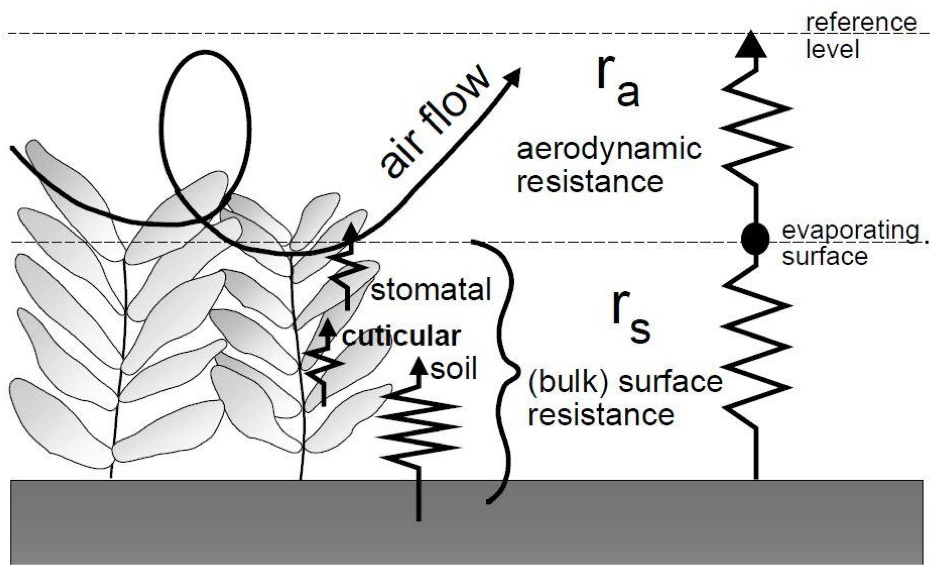
\includegraphics[width=0.8\textwidth]{figures/penman_widerstand.jpg}
\caption{Schematische Darstellung des aerodynamischen und des Oberflächenwiderstands in der Penman-Monteith-Methode}
\label{fig:widerstand}
\end{figure}

Der aerodynamische Widerstand beschreibt die Grösse, welche Wärme und Wasserdampf daran hindert , wegtransportiert zu werden. Diese hängt von der Windgeschwindigkeit und der Bodenrauigkeit ab. Der Oberflächenwiderstand beschreibt den Widerstand des Wasserdampfes, sich zwischen den transpirierenden Pflanzen und dem evaporierendem Boden zu bewegen. Dieser ist abhängig von Verhältnis der Blattfläche zur Bodenfläche und dem Stomatawiderstand eines gut bestrahlten Blattes. Unter Berücksichtigung dieser Einflüsse folgt die FAO\,Penman-Monteith-Formel für die Referenzfäche:

\begin{equation}
\label{eq:penman_ref}
ET_0=\frac{0.408\Delta \left(R_n-G\right)+\gamma \frac{900}{T+273}u_2\left(e_s-e_a\right)}{\Delta +\gamma\left(1+0.34u_2\right)}
\end{equation}
\begin{table}[H]
\centering
\begin{tabular}{ll}
$\mathrm{ET_0}$ & potentielle Referenzevapotranspiration $\mathrm{[mm/d]}$\\
$\mathrm{R_n}$ & Nettostrahlung $\mathrm{[MJ/m^2d]}$ \\
$\mathrm{G}$ & Bodenwärmefluss $\mathrm{[MJ/m^2d]}$\\
$\mathrm{\Delta}$ & Steigung der Sättigungsdampfdruckkurve $\mathrm{[kPa/^{\circ}C]}$\\
$\mathrm{\gamma}$ & Psychrometerkonstante $\mathrm{[kPa/^{\circ}C]}$\\
$\mathrm{T}$ & mittlere Temperatur in 2\,m Höhe $\mathrm{[^{\circ}C]}$\\
$\mathrm{u_2}$ & Windgeschwindigkeit in 2\,m Höhe $\mathrm{[m/s]}$\\
$\mathrm{e_s}$ & Sättigungsdampfdruck $\mathrm{[kPa]}$\\
$\mathrm{e_a}$ & aktueller Dampfdruck [kPa]\\
\end{tabular}
\end{table}

In den folgenden Berechnungen wird der Bodenwärmefluss allerdings vernachlässigt. Um die Evapotranspiration einer spezifischen Pflanze zu bestimmen, wird die Referenzevapotranspiration mit einem Pflanzenfaktor multipliziert. Es folgt daraus:

\begin{equation}
\label{eq:penman_spez}
ET_C=K_C*ET_0
\end{equation}
\begin{table}[H]
\centering
\begin{tabular}{ll}
$\mathrm{ET_0}$ & potentielle Referenzevapotranspiration $\mathrm{[mm/s]}$\\
$\mathrm{K_C}$ & Pflanzenfaktor [-]\\
$\mathrm{ET_C}$ & Evapotranspiration einer spezifischen Pflanze $\mathrm{[mm/s]}$\\\
\end{tabular}
\end{table}

Die Temperatur T kann aus den Meteodaten entnommen werden. Die übrigen Parameter müssen berechnet werden. Die FAO\,\cite{fao} gibt folgende Formeln:

\begin{description}
\item[Steigung der Sättigungsdampfdruckkurve]
\begin{equation}
\label{eq:delta}
\Delta=\frac{4098\left[0.6108*e^{\frac{17.27*T}{T+237.3}}\right]}{\left(T+237.3\right)^2}
\end{equation}
\begin{table}[H]
\centering
\begin{tabular}{ll}
$\mathrm{\Delta}$ & Steigung der Sättigungsdampfdruckkurve $\mathrm{[kPa/^{\circ}C]}$\\
T & mittlere Temperatur in 2\,m Höhe $\mathrm{[^{\circ}C]}$\\
\end{tabular}
\end{table}

\item[Nettostrahlung]
\begin{equation}
\label{eq:rn}
R_n=0.77*R_s-\sigma\left[\frac{T_{max,K}^4+T_{min,K}^4}{2}\right]\left(0.34-0.14\sqrt{e_a}\right)\left(1.35\frac{R_s}{R_{s0}}-0.35\right)
\end{equation}
\begin{table}[H]
\centering
\begin{tabular}{ll}
$\mathrm{R_n}$ & Nettostrahlung $\mathrm{[MJ/m^2d]}$ \\
$\mathrm{R_s}$ & Kurzwellenstrahlung $\mathrm{[MJ/m^2d]}$ \\
$\mathrm{\sigma}$ & Stefan Boltzmann Konstante $\mathrm{[4.903*10^{-9}\,MJ/K^4m^2d]}$\\
$\mathrm{T_{max,K}}$ & maximale Temperatur während 24 h [K]\\
$\mathrm{T_{min,K}}$ & minimale Temperatur während 24 h [K]\\
$\mathrm{e_a}$ & aktueller Dampfdruck [kPa]\\
$\mathrm{R_{s0}}$ & Kurzwellenstrahlung ohne Wolkenbedeckung $\mathrm{[MJ/m^2d]}$\\
\end{tabular}
\end{table}

\begin{equation}
\label{eq:rs0}
R_{s0}=\left(0.75+2*10^{-5}z\right)*R_a
\end{equation}
\begin{table}[H]
\centering
\begin{tabular}{ll}
$\mathrm{R_s0}$ & Kurzwellenstrahlung ohne Wolkenbedeckung $\mathrm{[MJ/m^2d]}$\\
$\mathrm{R_a}$ & extraterrestrische Strahlung $\mathrm{[MJ/m^2d]}$ \\
z & Höhe über Meer [m]\\
\end{tabular}
\end{table}

\begin{equation}
\label{eq:Ra_short_period}
R_{a}=\frac{12 (60)}{\pi}G_{sc}*d_{r}[(\omega _{2}-\omega _{1})sin(\varphi)sin(\delta)+cos(\varphi)cos(\delta)(sin(\omega _{2})- sin(\omega _{1}))]
\end{equation}
\begin{table}[H]
\centering
\begin{tabular}{ll}
R$\mathrm{_{a}}$ & extraterrestrische Strahlung in einer Stunde (oder in kürzerem Zeitintervall ) [MJ/m$\mathrm{^{2}}$h]\\
G$\mathrm{_{sc}}$ & Solarkonstante = 0.0820 MJ/m$\mathrm{^{2}}$min\\
d$\mathrm{_{r}}$ & inverse relative Distanz Sonne-Erde\\
$\mathrm{\delta}$ & solare Deklination [rad]\\
$\mathrm{\varphi}$ & geografische Breite [rad]\\
$\mathrm{\omega_{1}}$ & Sonneneinstrahlwinkel am Anfang der Zeitperiode [rad]\\
$\mathrm{\omega_{2}}$ & Sonneneinstrahlwinkel am Ende der Zeitperiode [rad]\\
\end{tabular}
\end{table}

\begin{equation}
\label{eq:Ra_long_period}
R_{a}=\frac{24 (60)}{\pi}G_{sc}*d_{r}[\omega _{s}sin(\varphi)sin(\delta)+cos(\varphi)cos(\delta)sin(\omega _{s}]
\end{equation}
\begin{table}[H]
\centering
\begin{tabular}{ll}
R$\mathrm{_{a}}$ & extraterrestrische Strahlung in einer Stunde (oder in kürzerem Zeitintervall ) [MJ/m$\mathrm{^{2}}$h]\\
G$\mathrm{_{sc}}$ & Solarkonstante = 0.0820 MJ/m$\mathrm{^{2}}$min\\
d$\mathrm{_{r}}$ & inverse relative Distanz Sonne-Erde\\
$\mathrm{\delta}$ & solare Deklination [rad]\\
$\mathrm{\varphi}$ & geografische Breite [rad]\\
$\mathrm{\omega_{s}}$ & Sonneneinstrahlwinkel [rad]\\
\end{tabular}
\end{table}



\item[Psychrometerkonstante]
\begin{equation}
\label{eq:gamma}
\gamma=0.665*10^{-3} P
\end{equation}
\begin{table}[H]
\centering
\begin{tabular}{ll}
$\mathrm{\gamma}$ & Psychrometerkonstante $\mathrm{[kPa/^{\circ}C]}$\\
P & Atmosphärendruck [kPa]\\
\end{tabular}
\end{table}

\item[Windgeschwindigkeit in 2 m Höhe]
\begin{equation}
\label{eq:u2}
u_2=u_z\frac{4.87}{ln(67.8z-5.42)}
\end{equation}
\begin{table}[H]
\centering
\begin{tabular}{ll}
$\mathrm{u_2}$ & Windgeschwindigkeit in 2\,m Höhe $\mathrm{[m/s]}$\\
$\mathrm{u_z}$ & Windgeschwindigkeit in z\,m Höhe $\mathrm{[m/s]}$\\
z & Messhöhe [m]\\
\end{tabular}
\end{table}

\item[Sättigungsdampfdruck]
\begin{equation}
\label{eq:es}
e_s=0.6108*e^{\frac{17.27T}{T+273.3}}
\end{equation}
\begin{table}[H]
\centering
\begin{tabular}{ll}
$\mathrm{e_s}$ & Sättigungsdampfdruck $\mathrm{[kPa]}$\\
T & mittlere Temperatur in 2\,m Höhe $\mathrm{[^{\circ}C]}$\\\end{tabular}
\end{table}

\end{description}

\subsection{Turc-Methode}
Das Modell von Turc ist für Frankreich und Nordafrika entwickelt worden und ist nur für Temperaturen über $\mathrm{^{\circ}C}$ definiert.

Es ist ein strahlungsbasiertes empirisches Modell. Als Input Parameter wird aber nicht nur die globale Strahlung, sondern auch die Temperatur benötigt. Das Modell ist nur für Temperaturen im positiven Bereich anwendbar und wird ungenau bei tiefen Temperaturen. Die potentielle Evapotranspirationsrate berechnet sich zu:

\begin{equation}
\label{eq:turc}
PET=0.31*C*\left(R_G+2.094\right)*\frac{T}{T+15}
\end{equation}
\begin{table}[H]
\centering
\begin{tabular}{ll}
PET & Evapotranspirationsrate nach Turc  $\mathrm{[mm/d]}$\\
T & mittlere Lufttemperatur im gegebenen Zeitinterval $\mathrm{{\circ}C]}$\\
$\mathrm{R_G}$ & globale Strahlung $\mathrm{[MJ/m^2\,d]}$\\
C & für rel. Luftfeuchtigkeit RH $\geq$ 50\% = 1\\
\end{tabular}
\end{table}
Für eine rel. Luftfeuchtigkeit < 50\% gilt:
\begin{equation}
\label{eq:turc_c}
C=1+\left(\frac{50-RH}{70}\right)
\end{equation}
\begin{table}[H]
\centering
\begin{tabular}{ll}
RH& durchschnittliche rel. Luftfeuchtigkeit [\%]\\
\end{tabular}
\end{table}

\subsection{Ivanov-Methode}
Das Modell von Ivanov ist eine modifizierte Version des Modells von Turc. Es kann für die Abschätzung der Evapotranspirationsrate bei tieferen Temperaturen in den Monaten November bis Februar genutzt werden und ist ein temperaturbasiertes Modell. Für die Berechnung der täglichen Evapotranspiration wird folgende Formel benutzt:

\begin{equation}
\label{eq:ivanov_d}
PET=0.000036*(25+T)^2*(100-RH)
\end{equation}
\begin{table}[H]
\centering
\begin{tabular}{ll}
PET & Evapotranspirationsrate nach Ivanov  $\mathrm{[mm/d]}$\\
T & mittlere Lufttemperatur im gegebenen Zeitinterval $\mathrm{{^\circ}C]}$\\
$\mathrm{R_G}$ & globale Strahlung $\mathrm{[MJ/m^2\,d]}$\\
\end{tabular}
\end{table}

Für die monatliche Evapotranspiration wird folgende Formel verwendet:

\begin{equation}
\label{eq:ivanov_m}
PET=0.0011*(25+T)^2*(100-RH)
\end{equation}
\begin{table}[H]
\centering
\begin{tabular}{ll}
PET & Evapotranspirationsrate nach Ivanov  $\mathrm{[mm/Mt]}$\\
T & mittlere Lufttemperatur im gegebenen Zeitinterval $\mathrm{{^\circ}C]}$\\
$\mathrm{R_G}$ & globale Strahlung $\mathrm{[MJ/m^2\,d]}$\\
\end{tabular}
\end{table}







\section{Resultate}




\subsection{Sensitivitätsanalyse}
Die Penman-Montheit Methode zeigt die grösste Sensitivität gegenüber des Sättigungsdampfdruckes. Die Veränderungen von Niederschlagsmenge, relativer Luftfeuchtigkeit und Sonnenscheindauer zeigen kaum eine Änderung der Evapotranspiration. Die Methode nach Turc zeigt die grösste Sensitivität gegenüber der relativen Luftfeuchtigkeit und die Lufttemperatur hat den kleinsten Einfluss. Die Methode nach Ivanov reagiert auf beide Parameter Lufttemperatur und relative Luftfeuchtigkeit etwa gleich empfindlich. Die genauen Resultate und die Berechnung ist im Anhang\,\ref{sec:sensitivitaet} ersichtlich.
\section{Diskussion}




\subsection{Sensitivitätsanalyse}
Die Sensitivitätsanalyse der Penman-Monteith Methode zeigt, dass der Sättigungsdampfdruck den grössten Einfluss auf die Evapotranspiration hat und die Grösse Bodentemperatur invers auf das Resultat Einfluss nimmt. Die Analyse zeigt auch, dass Niederschlag, relative Luftfeuchtigkeit und Sonnenscheindauer vernachlässigbar sind. Dies ist allerdings fragwürdig, da der Niederschlag der limitierende Faktor der Evapotranspiration ist. <<

Bei der Methode nach Turc ist bereits aus der Formel (\ref{eq:turc}) ersichtlich, dass die relative Luftfeuchtigkeit linear in die Berechnung der Evapotranspiration eingeht und somit auch den Grössten Einfluss auf das Resultat hat. Die anderen Grössen fliessen nicht linear ein, was auch die Sensitivitätsanalyse widerspiegelt.

Die Methode nacht Ivanov zeigt bei tiefen Temperaturen eine ausgeglichene Sensitivität auf die beiden Parameter. Für höhere Temperaturen reagiert die Evapotranspiration allerdings sehr viel sensitiver auf die Lufttemperaturen. 

\begin{appendix}

\section{Sensitivitätsanalyse}
\label{sec:sensitivitaet}



\end{appendix}


% für Literaturverzeichnis
\bibliographystyle{natdin}
\bibliography{experiment4}


\end{document}

$ latex myarticle
$ bibtex myarticle
$ latex myarticle
$ latex myarticle
